\documentclass[tikz,border=2pt]{standalone}
\usepackage{amsmath,amssymb}
\usepackage{tikz}
\usetikzlibrary{arrows.meta}

\begin{document}
% R^2 with the dot product: lengths from Pythagoras, distances as lengths of differences,
% and angles from <x,y> = ||x|| ||y|| cos θ.
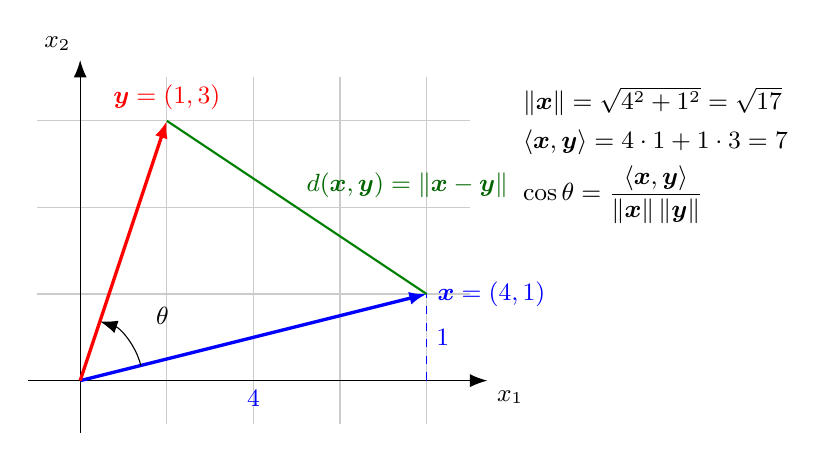
\begin{tikzpicture}[scale=1.1, every node/.style={font=\small}, >={Latex[length=2.2mm]}]
	\draw[gray!40, step=1] (-0.5,-0.5) grid (4.5,3.5);
	\draw[->] (-0.6,0) -- (4.7,0) node[below right] {$x_1$};
	\draw[->] (0,-0.6) -- (0,3.7) node[above left] {$x_2$};
	\draw[->, blue, very thick] (0,0) -- (4,1) node[right] {$\boldsymbol{x}=(4,1)$};
	\draw[->, red, very thick] (0,0) -- (1,3) node[above] {$\boldsymbol{y}=(1,3)$};
	\draw[dashed, blue] (4,0) -- (4,1);
	\node[blue, below] at (2,0) {$4$}; \node[blue, right] at (4,0.5) {$1$};
	\draw[green!50!black, thick] (4,1) -- (1,3);
	\node[green!40!black, above right] at (2.5,2.0) {$d(\boldsymbol{x},\boldsymbol{y})=\|\boldsymbol{x}-\boldsymbol{y}\|$};
	\draw[->, black] (0.7,0.175) arc (14:71.6:0.72);
	\node at (0.95,0.75) {$\theta$};
	\node[anchor=west, align=left] at (5.0,2.6) {$\|\boldsymbol{x}\|=\sqrt{4^2+1^2}=\sqrt{17}$\\[3pt] $\langle\boldsymbol{x},\boldsymbol{y}\rangle=4\cdot1+1\cdot3=7$\\[3pt] $\cos\theta=\dfrac{\langle\boldsymbol{x},\boldsymbol{y}\rangle}{\|\boldsymbol{x}\|\,\|\boldsymbol{y}\|}$};
\end{tikzpicture}
\end{document}
